\documentclass[acmtog]{acmart}
\usepackage{graphicx}
\usepackage{subfigure}
\usepackage{natbib}
\usepackage{listings}
\usepackage{bm}
\usepackage{amsmath}

\definecolor{blve}{rgb}{0.3372549 , 0.61176471, 0.83921569}
\definecolor{gr33n}{rgb}{0.29019608, 0.7372549, 0.64705882}
\makeatletter
\lst@InstallKeywords k{class}{classstyle}\slshape{classstyle}{}ld
\makeatother
\lstset{language=C++,
	basicstyle=\ttfamily,
	keywordstyle=\color{blve}\ttfamily,
	stringstyle=\color{red}\ttfamily,
	commentstyle=\color{magenta}\ttfamily,
	morecomment=[l][\color{magenta}]{\#},
	classstyle = \bfseries\color{gr33n}, 
	tabsize=2
}
\lstset{basicstyle=\ttfamily}

% Title portion
\title{Assignment 1:\\ {Exploring OpenGL and Phong Lighting}} 

\author{Name:\quad Entropy-Fighter\\ student number:\ 2020533
\\email:\quad xxxx@shanghaitech.edu.cn}

% Document starts
\begin{document}
\maketitle

\vspace*{2 ex}

\section{Introduction}
\quad
In Assignment1, we are required to construct the objects(plane, bunny, sphere) from the given information and render them with Phong lighting model.
In this homework, I do the following things.
\begin{itemize}
\item Load different objects' meshes from obj files and draw them.
\item Use Phong lighting model to make objects appear to be 3D.
\item Use mouse and keyboard to control the camera.

\item Carry a Flashlight (Spot Light) with the camera. (optional part)
\item Use geometry shader to make fur for the bunny. (optional part)
\end{itemize}

\section{Implementation Details}

\subsection{Load Meshes From Obj Files}
\quad
This part is implemented in the function "loadDataFromFile" in "scr/mesh.cpp". 
I use ifstream and stringstream to load information from the objectfiles. Then, I store the vertex information 
in "std::vector<Vertex> vertices", which is a vertex vector containing position and normal information for per vertex. 
Also, I store the mesh information in "std::vector<GLuint> indices", which is a GLuint vector containing the indices of vertices for each triangle.
When I creat the Mesh object, it would call this loadDataFromFile function, which prepares mesh information for the next drawing and rendering.

\subsection{Draw Meshes}


\subsubsection{Preparing work: VBO, VAO and EBO}
~

This part is implemented in the function "prepare" in "scr/mesh.cpp". 
The steps to build VBO and EBO are similar. Let me take the VBO as example. 
Firstly, we need to generate a VBO object, then we bind vertex buffer object to the target(GL\_ARRAY\_BUFFER).
After binding, on any buffer calls we make (on the GL\_ARRAY\_BUFFER target) will be used to configure the currently bound buffer, which is VBO. 
Then, we copy vertex data to buffer's memory using function glBufferData.
This means our VBO now contains the data of "std::vector<Vertex> vertices", which has vertex attributes.

Building EBO is similar, but EBO stores indices that OpenGL uses to decide what vertices to draw rather than the vertices like VBO. We can do indexed drawing if we use EBO.

As for VAO, in my view, it is more like a manager who manages VBO and EBO. To make it more clear, I take some notes and pictures about VAO from "https://learnopengl.com/Getting-started/Hello-Triangle" as reference. 
\begin{figure}[h]
	\centering
	{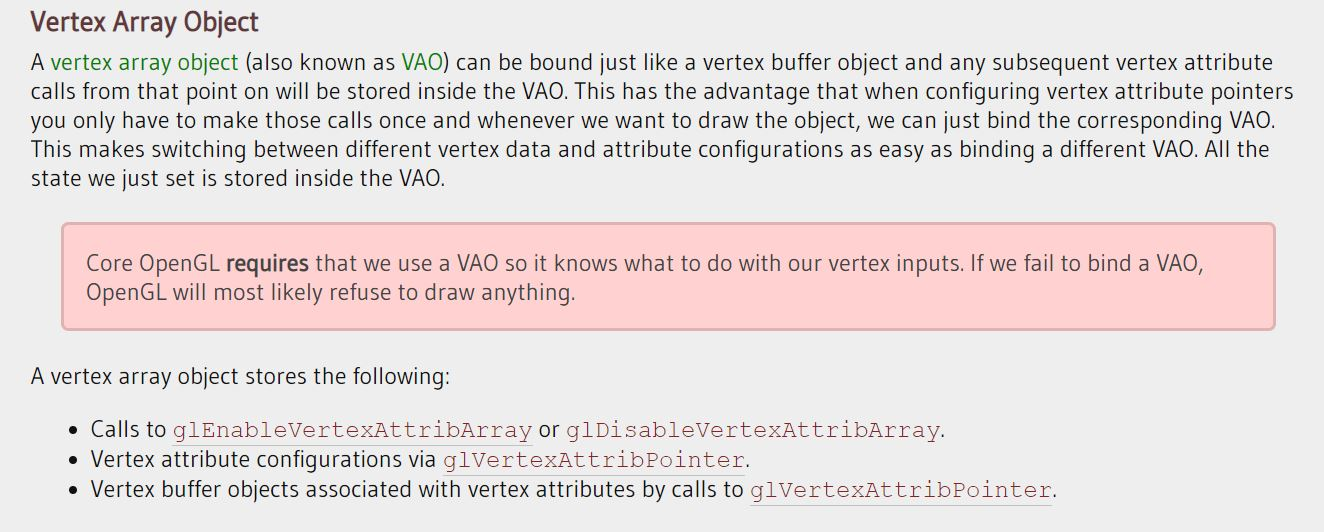
\includegraphics[width=8cm]{VAO.JPG}}
	{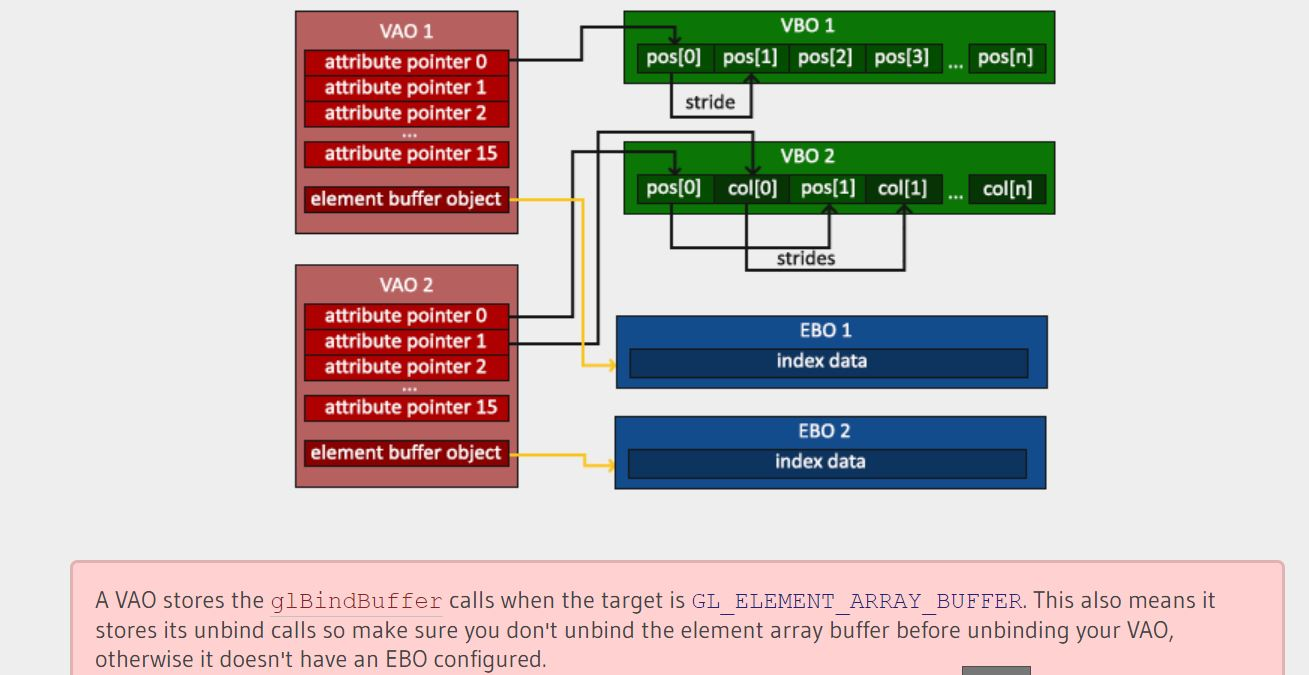
\includegraphics[width=8cm]{VAO_graph.JPG}}
\end{figure}

When building the VAO, the most important step is to configure the vertex attributes using glVertexAttribPointer. We have to set the layout position, step size and offset properly. 


\subsubsection{Vertex Shader and Fragment Shader}
~

Shaders are little programs that rest on the GPU. These programs are run for each specific section of the graphics pipeline, transforming inputs to outputs according to our needs.

Vertex shader and fragment shader are often used in the rending process. I write my shaders in ".fs" and ".vs" files in shaderSourceCode folder.

Our vertex shader gets data from VBO. "layout", as it means, is used to tell the shader the layout of vertex attributes in VBO. In our case, we get vertex position and normal as our vertex shader's inputs.

It seems that the vertex information we get from the VBO is enough for us to draw a 3D objects. However, the inforamtion is just in local space. We hope we can get vertex information in clip space from the outputs of vertex shader, so we should do some transformations.
The model matrix transforms the vertex coordinates from local space to world space. I set the identical matrix since I just want to draw one object each time.

The view matrix transforms the coordinates from world space to view space. The view matrix can be generated by glm:lookAt, we only need to pass 3 directional vectors of camera(eyes) to it, which are cameraPos, cameraPos + cameraFront and cameraUp.

The projection matrix transforms the coordinates from view space to clip space. In our case, we hope to do the perspective projection, so the matrix can be generated by glm:perspective. We need to pass fov(field of view), aspect ratio(w/h), distance to near clip plane and distance to far clip plane to the function.

These matrices are created in "main.cpp", we transfer them to our vertex shader by using uniforms. Uniforms are another way to pass data from application on the CPU to the shaders on the GPU, but they are slightly different from vertex attributes. They are always global. We set unifrom variables simply by using the setMat4 function in Shader class offered by TAs.
In vertex shader source code, we only need to add keyword "uniform" to these 3 variables.
Finally, these 3 matrices are applied to vertex position and we assign the transformed position to "gl\_Position".

Fragment shader, as its name implies, is used to render fragments. In the most simple case, it should has the output frag\_color. We will talk about more complex implementation of fragment shader in phong lighing model section.


\subsubsection{Shader Class}
~

Fortunately, the teaching group has implemented most of the shader class in "shader.cpp". We only need to complete the initWithCode function, which dynamicly compiles the shader source code. 

In order to compile shaders, we should firstly create shader objects, referenced by IDs, then attach the shader source codes to the shader objects and compile them. Also, we need to check for compile-time errors.
At last, we should use the glCreateProgram function to create a program and return the ID reference to the newly created shader program, then we attach the shader objects to the shader program and link them.

~

After implementing 2.2.1, 2.2.2 and 2.2.3, we can now draw the meshes. This part is implemented in the draw function in mesh.cpp, which binds VAO and uses glDrawElements to draw the meshes.
Then, in the rendering "while loop" in "main.cpp", we just need to call the shader program's use function and the mesh object's draw function.

\subsection{Use Phong Lighting Model}
\quad
So far, our objects only have shapes and do not appear to be 3D. Therefore, we have to add some shadows and lights using phong lighting model.
What we need to do is to modify the fragment shader. 

As we all know, phong lighting model has 3 components: ambient light, diffuse Light and specular light. We will talk about them successively.
\subsubsection{Ambient Light}
~

Ambient light comes from the environment around us. 
To simulate this, we set a small constant ambient factor. Here, I set the ambient\_factor to 0.1.
Then, we take the light's color, multiply it with this ambient\_factor, and use that as the ambient light.


\subsubsection{Diffuse Light}
~

When calculating diffuse light, we need to know light position and normal.
Therefore, in vertex shader, we should output light position and normal. Then, in fragment shader, we get these two outputs as inputs.

Now, we have to calculate dot product of light direction vector and normal vector, and multiply it with ligth\_color to get diffuse light.

\subsubsection{Specular Light}
~

In diffuse light section, we already know the light direction and normal. 
Then, we use reflect function to calculate the reflected light direction vector. Also, we need to calculate the view direction vector using frag\_position and camera\_position.
The next step is to calculate the dot product between the view direction and the reflect direction (it's non-negative) and then raise it to the power of 32. This 32 value is the shininess value of the highlight.
At last, we multiply this with light color and a specular intensity value to get specular light.

~

After calculating ambient light, diffuse light and specular light, we just add them and multiply it with the color of object to get frag\_color.
So far, when we draw meshes, we can make our objects appear to be 3D.

\subsection{Control the Camera}

In this section, we hope our camera view to be more flexible. Therefore, I do the following things.
\begin{itemize}
\item move the camera up and down by pressing "W" and "S".
\item move the camera left or right by pressing "A" and "D".
\item change pitch and yaw of camera by mouse.
\item implement a zooming interface by scrolling.
\end{itemize}

\subsubsection{Control the camera by keyboard}
~

This part is implemented in process\_input function in "main.cpp".
This function can get "ESC" keyboard input to exit the rendering loop.
Also, it can get "W", "S", "A", "D" keyboard inputs to change the camera position by changing relevant camera vector and corresponding view matrix. 

In order to make our camera speed balanced in all machines, we have to calculate delta\_time, which is the time interval between last frame and current frame.
Then we set our camera speed to be the delta\_time multiplying one constant.

\subsubsection{Control the camera by mouse}
~

This part is implemented in mouse\_callback function in "main.cpp".
In mouse\_callback function, we have to calculate the offset of the moving mouse on x and y direction and change the "yaw" and "pitch" of camera.
Then we need to modify the cameraFront vector and corresponding view matrix.

In order to implement a zooming interface, I add the scroll\_callback function in "main.cpp". This function is to change the fov by scrolling.

After we complete these 2 callback functions, we still need to do somthing in main function. 
Firstly we should tell GLFW that it should hide the cursor and capture it, then we should tell GLFW to listen to mouse-movement and mouse-scrolling events. 
After doing these, we have a much more flexible camera.

\subsection{Carry a Flashlight with the Camera(optional)}
\quad
Now, we want to carry a flashlight with the camera. Therefore, we should re-design the fragment shader.

In order to implement spot light, we need to add 3 new uniform variables, which are cutoff, outer\_cutoff and cone\_direction.
The cutoff angle specifies the spotlight's radius. Everything outside cutoff angle can not be lit by the spotlight.
Outer\_cutoff is used to construct smooth edges, and cone\_direction meanss the spot direction. 
We want to find out the angle between the light direction vector and the cone\_direction vector, and this angle cannot be larger than the cutoff angle. 

By intensity formula and clamp function, we can quickly calculate intensity. What we need to do is to make diffuse and specular light multiply this intensity.
Also, we should set the light direction to the camera direnction and set the light position to the camera position.
(In this section, I also add attenuation to fragment shader, which makes the light more true to life.)
\subsection{Use Geometry Shader to Make Fur for the Bunny(optional)}
\quad
Firstly, we should modify the shader class. We have to read the ".gs" file and compile the geometry shader. It is similar to 2.2.3. 

Next, we should design our "fur.gs" file. 
Geometry shader is between the vertex and the fragment shader.
A geometry shader takes as input a set of vertices that form a single primitive. The geometry shader can then transform these vertices as it sees fit before sending them to the next shader stage. 

The interesting thing about gs is that it is able to convert the original set of vertices to different primitives.
What we want to do is replace the original mesh triangle to a tetrahedron, in which case our bunny would seem to have fur.
Therefore, we should generate a new vertex. Using this new vertex and the 3 original vertices, the geometry shader can generate a fake tetrahedron.
\section{Results}
% pictures should be in
\begin{figure}[h]
	\centering
	\subfigure[bunny]
	{
		\begin{minipage}[b]{.4\linewidth}
		\centering
		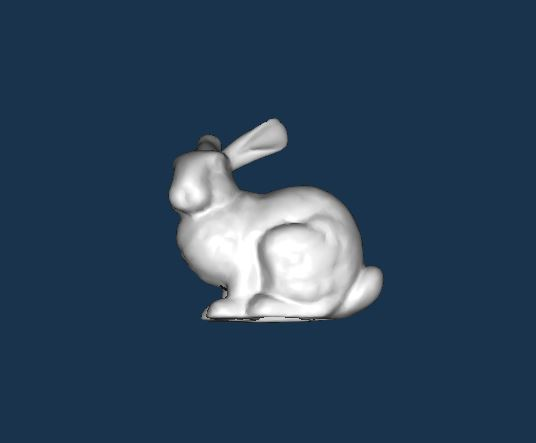
\includegraphics[width = 3cm]{bunny.JPG}
		\end{minipage}
	}
	\subfigure[sphere]
	{
		\begin{minipage}[b]{.4\linewidth}
		\centering
		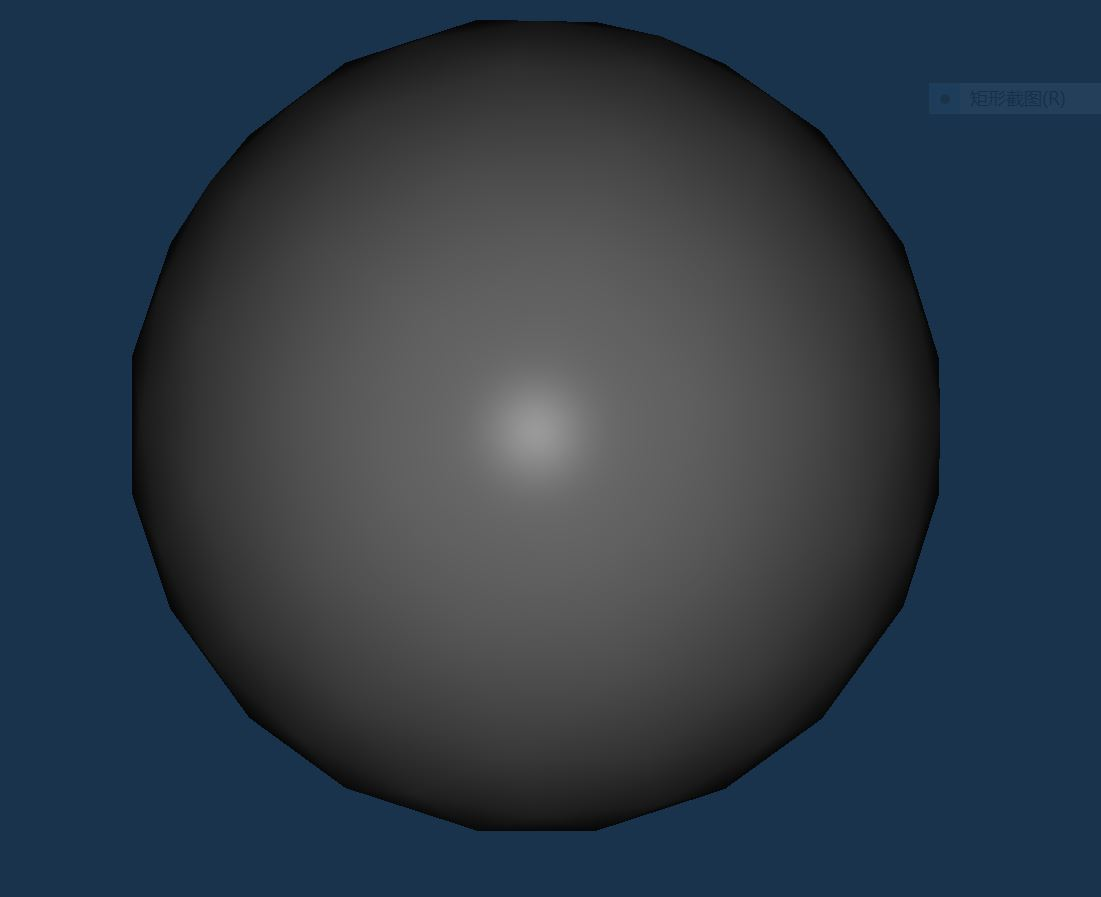
\includegraphics[width = 3cm]{sphere.JPG}
		\end{minipage}
	}

	\subfigure[plane] 
	{
		\begin{minipage}[b]{.4\linewidth}
		\centering
		
\includegraphics[width = 3cm]{plane.JPG}
		\end{minipage}
	}
	\subfigure[use spot light]
	{
		\begin{minipage}[b]{.4\linewidth}
		\centering
		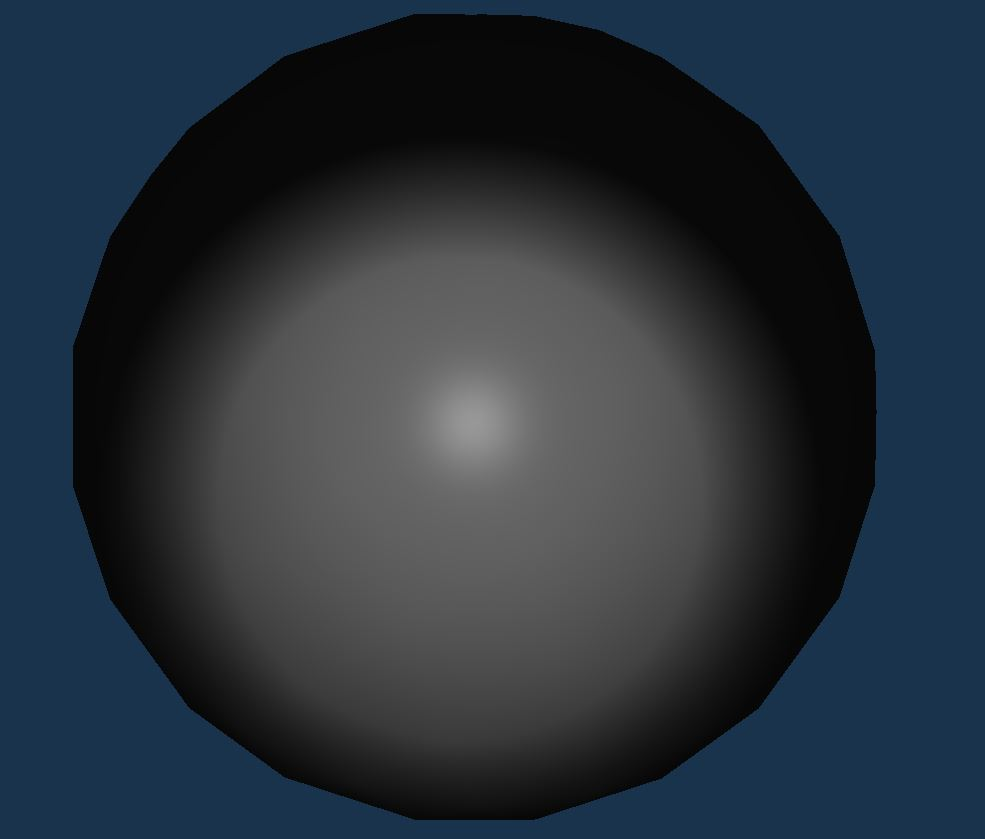
\includegraphics[width = 3cm]{spot_light1.JPG}
		\end{minipage}
	}
	\subfigure[use spot light with camera]
	{
		\begin{minipage}[b]{.4\linewidth}
		\centering
		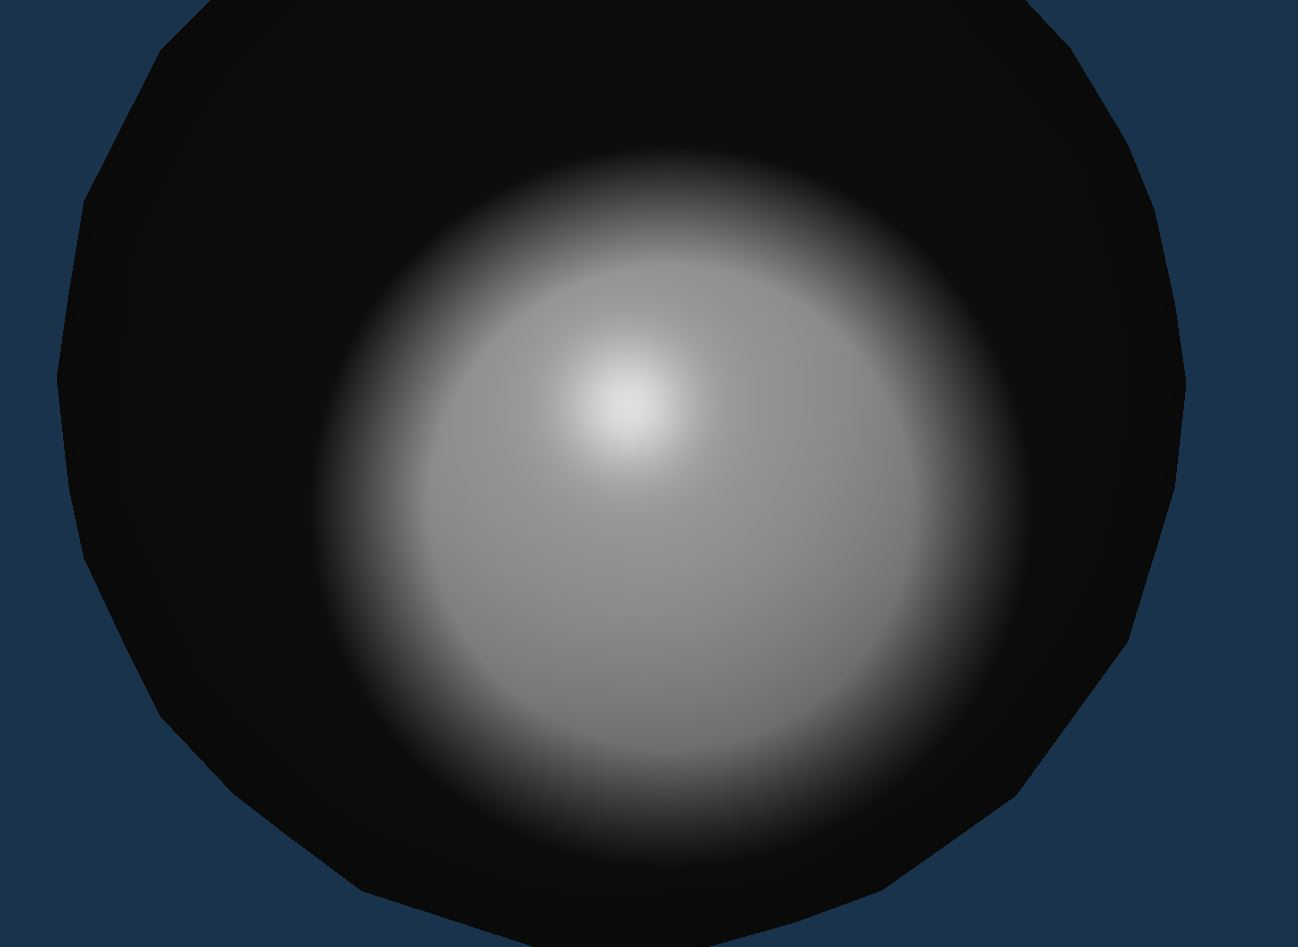
\includegraphics[width = 3cm]{spot_light2.JPG}
		\end{minipage}
	}
	\subfigure[bunny with fur]
	{
		\begin{minipage}[b]{.4\linewidth}
		\centering
		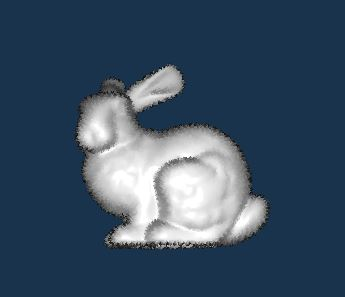
\includegraphics[width = 3cm]{fur_bunny.JPG}
		\end{minipage}
	}
	\end{figure}

\end{document}